
\begin{center}
    \tikzstyle{myclass} = [rectangle, draw, text centered]
    \tikzstyle{line} = [draw, -latex, line width=.1em]

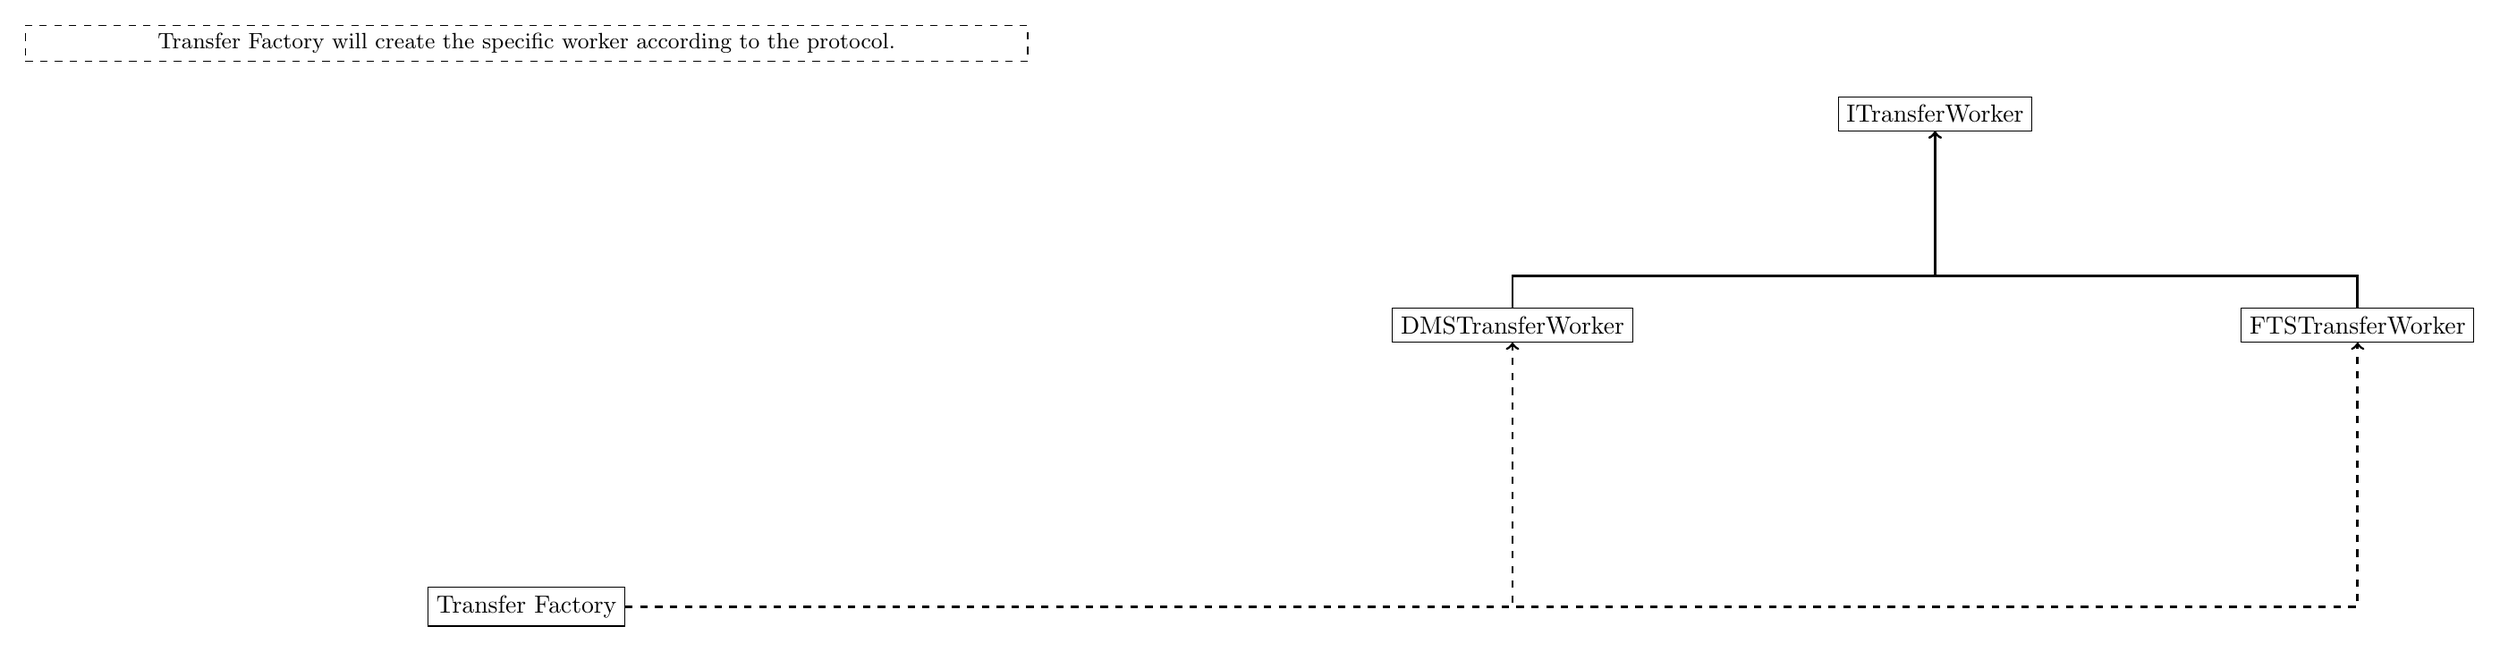
\begin{tikzpicture}[scale=0.9]
    \node[myclass](ITransferWorker){ITransferWorker};
    \node[below of=ITransferWorker, node distance=3cm](DummyWorker){};
    \node[myclass,left of=DummyWorker, node distance=6cm]
            (DIRACDMSTW){DMSTransferWorker};
    \node[myclass,right of=DummyWorker, node distance=6cm]
            (DIRACFTSTW){FTSTransferWorker};
    \node[below of=DummyWorker, node distance=4cm](DummyWorker2){};
    \node[myclass, left of=DummyWorker2, node distance=20cm]
            (TransFactory){Transfer Factory};

    \node[myclass, above of=TransFactory,dashed, node distance=8cm,
          font=\small, text width=14cm]
            (FactoryMemo){
            Transfer Factory will create the specific worker
            according to the protocol.
        };

    \path[line,->](DIRACDMSTW.north) -- ++(0,0.5) -| (ITransferWorker.south);
    \path[line,->](DIRACFTSTW.north) -- ++(0,0.5) -| (ITransferWorker.south);

    \path[line,dashed,->](TransFactory.east) -| (DIRACDMSTW.south);
    \path[line,dashed,->](TransFactory.east) -| (DIRACFTSTW.south);
\end{tikzpicture}
\end{center}
